\documentclass[a4paper,12pt]{ctexart}
\usepackage[utf8]{inputenc}
\usepackage{geometry}
\usepackage{graphicx}
\usepackage{float}
\usepackage{booktabs}
\usepackage{amsmath}
\usepackage{amssymb}
\usepackage{hyperref}
\usepackage{listings}
\usepackage{xcolor}
\usepackage{caption}
\usepackage{subcaption}
\usepackage{multirow}
\usepackage{array}

\geometry{left=2.5cm,right=2.5cm,top=2.5cm,bottom=2.5cm}

\title{\textbf{ESC-50 环境声音检索与分类系统报告}}
\author{数字信号处理课程大作业}
\date{\today}

% 代码高亮设置
\lstset{
    basicstyle=\ttfamily\small,
    keywordstyle=\color{blue},
    commentstyle=\color{gray},
    stringstyle=\color{purple},
    breaklines=true,
    frame=single,
    numbers=left,
    numberstyle=\tiny,
    xleftmargin=2em
}

\begin{document}

\maketitle

\begin{abstract}
本报告详细阐述了基于ESC-50数据集的环境声音检索与分类系统的设计与实现。项目采用“从零构建”的理念,手动实现了快速傅里叶变换(FFT)、短时傅里叶变换(STFT)及梅尔频率倒谱系数(MFCC)等核心DSP算法,深入理解了频域分析的数学本质。在此基础上,构建了基于MFCC特征的无监督检索系统,并设计了ResNet风格的卷积神经网络(CNN)进行有监督分类,实现了75.00\%的测试准确率。进一步地,项目引入了PANNs、AST、CLAP等前沿预训练模型进行迁移学习对比,其中CLAP模型达到了97.25\%的分类精度。最后,本研究还探索了基于Gemini大语言模型和CLAP零样本学习的音频理解能力。实验结果不仅验证了经典信号处理方法的有效性,也展示了现代深度学习在音频领域的强大潜力,体现了从底层信号解析到高层语义理解的技术跨越。
\end{abstract}

\tableofcontents
\newpage

\section{引言}

环境声音识别(Environmental Sound Classification, ESC)是机器听觉领域的核心任务之一,旨在让计算机系统能够感知并理解周围环境中的非语言声音。与语音识别和音乐检索不同,环境声音通常具有非平稳性、背景噪声复杂、声源多样(如自然界声音、动物叫声、城市噪音等)的特点,这对信号处理和特征提取提出了更高的要求。

ESC-50 (Environmental Sound Classification 50) 是该领域的各类算法得标准评估基准。本项目以此为基础,构建了一套完整的音频分析系统。本项目的核心目标不仅在于追求高识别率,更在于通过“从底层算法到顶层应用”的完整实现,深入探讨数字信号处理(DSP)技术与现代人工智能(AI)模型的内在联系。

\section{数据集与实验环境}

\subsection{ESC-50 数据集概述}
ESC-50数据集由Karol Piczak于2015年发布,包含2000条带标注的环境音频片段。

\begin{table}[htbp]
\centering
\caption{ESC-50 数据集统计信息}
\label{tab:dataset_stats}
\begin{tabular}{ll}
\toprule
参数 & 描述 \\
\midrule
样本总数 & 2000条 \\
类别总数 & 50类(分为5大组) \\
每类样本数 & 40条 \\
音频时长 & 5秒 \\
采样率 & 44.1 kHz \\
数据格式 & 单声道 WAV \\
划分 & 5-Fold Cross Validation \\
\bottomrule
\end{tabular}
\end{table}

数据集的50个类别被划分为5个大类,涵盖了生活中常见的声音场景(见表\ref{tab:categories})。

\begin{table}[htbp]
\centering
\caption{ESC-50 类别分布}
\label{tab:categories}
\begin{tabular}{ll}
\toprule
大类 & 包含类别示例 \\
\midrule
动物声音 (Animals) & 狗叫、猫叫、猪叫、牛叫、鸟鸣等 \\
自然界声音 (Natural) & 雨声、海浪、风声、雷声、水流等 \\
人类非语音 (Human) & 咳嗽、喷嚏、呼吸、脚步声、笑声等 \\
室内声音 (Interior) & 敲门、键盘声、闹钟、吸尘器、玻璃破碎等 \\
城市/室外噪声 (Exterior) & 直升机、电锯、警笛、汽车喇叭、发动机等 \\
\bottomrule
\end{tabular}
\end{table}

\subsection{数据划分与预处理}
本项目严格遵循官方推荐的5折交叉验证:
\begin{itemize}
    \item 训练集/数据库:Fold 1-4 (1600条样本)。
    \item 测试集/查询集:Fold 5 (400条样本)。
\end{itemize}
在 DSP/MFCC 与 CNN 训练/检索流程中,音频通过 \texttt{load\_audio} 按配置采样率重采样(默认 44.1kHz,可在脚本参数中调整),并用 \texttt{normalize\_audio} 做峰值归一化到 [-1,1]。CLAP/Gemini 等则使用各自模型采样率。

\section{核心与基础:DSP算法实现及其物理意义}

傅里叶分析构成了音频信号处理的基石。在本项目中,我们没有调用现成的函数(如 `numpy.fft` 或 `librosa.stft`),而是选择手工实现每一行核心代码,以求彻底掌握其数学原理与物理意义。

\subsection{快速傅里叶变换 (FFT)}

傅里叶变换揭示了信号的时频二象性:任何时域信号都可以看作是不同频率正弦波的叠加。离散傅里叶变换(DFT)将这一思想数字化:
\begin{equation}
X[k] = \sum_{n=0}^{N-1} x[n] e^{-j2\pi kn/N}
\end{equation}
直接计算DFT的时间复杂度为$O(N^2)$。本项目实现了经典的\textbf{Cooley-Tukey Radix-2算法},利用旋转因子$W_N^{kn} = e^{-j2\pi kn/N}$的周期性和对称性,将DFT递归分解为偶数项和奇数项两部分:
\begin{equation}
X[k] = \text{DFT}_{N/2}\{x_{even}\}[k] + W_N^k \cdot \text{DFT}_{N/2}\{x_{odd}\}[k]
\end{equation}
通过递归分治,复杂度降低至$O(N\log N)$。

\textbf{算法实现细节:}
\begin{enumerate}
    \item \textbf{位反转置换 (Bit-reversal Permutation)}:为了实现原位运算(In-place),输入序列需要按索引的二进制位反转顺序重排。例如,$N=8$时,索引$1 (001_2)$变为$4 (100_2)$。
    \item \textbf{蝶形运算 (Butterfly Operation)}:核心计算单元,通过加减法结合旋转因子$W_N^k$完成两点DFT。
\end{enumerate}

我们通过与标准库`numpy.fft`对比验证了实现的精度,复数域相对误差仅为 $2.54 \times 10^{-8}$,证明了底层实现的准确性。

\subsection{短时傅里叶变换 (STFT)}

由于环境声音往往是非平稳的(例如狗叫声是间歇的,雨声是持续的),单纯的FFT无法描述频率随时间的变化。STFT引入了“时间窗”的概念,对信号分帧加窗处理:
\begin{equation}
STFT\{x[n]\}(m, \omega) = \sum_{n=-\infty}^{\infty} x[n]w[n-mH]e^{-j\omega n}
\end{equation}
其中$w[n]$为窗函数,$H$为帧移(Hop Length),$m$为帧索引。

本项目使用\textbf{Hann窗}以减少频谱泄露:
\begin{equation}
w[n] = 0.5 - 0.5 \cos\left(\frac{2\pi n}{N-1}\right), \quad 0 \le n \le N-1
\end{equation}

\textbf{物理意义:} STFT产生了一个二维的时频矩阵(频谱图)。这是一个包含丰富信息的图像数据,它打通了音频处理与计算机视觉(CV)的桥梁,使得我们后续能够使用卷积神经网络(CNN)来处理一维的声音信号。

\begin{figure}[htbp]
    \centering
    \includegraphics[width=0.9\textwidth]{figures/viz_stft.png}
    \caption{自定义STFT频谱图可视化(示例:Fireworks)}
    \label{fig:viz_stft}
\end{figure}

\subsection{梅尔频率倒谱系数 (MFCC)}

虽然STFT提供了完整的时频信息,但它并不符合人耳的听觉特性。人耳对频率的感知是非线性的(对低频更敏感)。MFCC通过以下步骤模拟这一特性:

\subsubsection{Log-Mel 频谱图}
在进行倒谱变换之前,我们需要先计算Log-Mel频谱图,这是许多现代深度学习模型(如所有的ResNet、AST、PANNs)的标准输入特征。

1. \textbf{预加重 (Pre-emphasis)}:使用滤波器 $y[n] = x[n] - \alpha x[n-1]$ ($\alpha=0.97$) 提升高频分量,平衡频谱能量。
2. \textbf{Mel滤波器组}:将线性频率$f$映射到Mel非线性尺度$m$:
\begin{equation}
m = 2595 \log_{10}\left(1 + \frac{f}{700}\right)
\end{equation}
在此尺度上设计三角滤波器组,计算每个滤波器的对数能量。

Log-Mel频谱图有效地压缩了频率维度(从1025维线性频率压缩到40-128维Mel频率),同时保留了人耳感知的关键信息。

\begin{figure}[htbp]
    \centering
    \includegraphics[width=0.9\textwidth]{figures/viz_logmel.png}
    \caption{自定义Log-Mel频谱图可视化(示例:Fireworks,40 Mels)}
    \label{fig:viz_logmel}
\end{figure}

\subsubsection{倒谱系数 (MFCC)}
为了去除频谱特征的相关性,我们对Log-Mel谱进行离散余弦变换 (DCT-II):
\begin{equation}
c[k] = 2 \sum_{n=0}^{N-1} x[n] \cos\left[ \frac{\pi}{N} \left(n+\frac{1}{2}\right) k \right]
\end{equation}
通常取前13维系数作为MFCC特征。

\begin{figure}[htbp]
    \centering
    \includegraphics[width=0.9\textwidth]{figures/viz_mfcc.png}
    \caption{自定义MFCC系数可视化(示例:Fireworks,13系数)}
    \label{fig:viz_mfcc}
\end{figure}

\textbf{数学与感知的桥梁:} MFCC舍弃了详细的细微末节,保留了声音的“包络”特征(共振峰结构),这对于区分音色(Timbre)至关重要。从图\ref{fig:viz_mfcc}中可以看出,MFCC的能量主要集中在低阶系数(底部),这反映了信号的主要频谱包络信息。

\section{任务一:基于MFCC的声音检索系统}

\subsection{系统设计}
检索系统的核心在于如何度量两个音频片段的相似性。我们采用MFCC作为特征载体:
\begin{itemize}
    \item \textbf{特征提取}:计算每一帧的13维MFCC系数。
    \item \textbf{特征聚合}:计算整个音频片段MFCC的均值向量(Mean)和标准差向量(Std),拼接得到26维的全局特征向量。这相当于捕捉了声音的平均音色和音色的变化范围。
    \item \textbf{相似度度量}:使用余弦相似度(Cosine Similarity)。
\end{itemize}

\subsection{实验结果:帧长与帧移的影响}
我们在不同的帧长(512-4096)和帧移(256-2048)下进行了全排列网格搜索实验。Top-10和Top-20的检索精度如表\ref{tab:retrieval_top10}和表\ref{tab:retrieval_top20}所示。

\begin{table}[htbp]
\centering
\caption{MFCC检索 Top-10 精度 (Frame Length vs Hop Length)}
\label{tab:retrieval_top10}
\begin{tabular}{c|cccc}
\toprule
\multirow{2}{*}{Frame Length} & \multicolumn{4}{c}{Hop Length} \\
 & 256 & 512 & 1024 & 2048 \\
\midrule
512  & 0.6500 & 0.6475 & 0.6450 & 0.6525 \\
1024 & 0.6575 & 0.6525 & 0.6525 & 0.6400 \\
2048 & \textbf{0.6775} & \textbf{0.6775} & 0.6625 & 0.6600 \\
4096 & 0.6575 & 0.6575 & 0.6625 & 0.6600 \\
\bottomrule
\end{tabular}
\end{table}

\begin{table}[htbp]
\centering
\caption{MFCC检索 Top-20 精度 (Frame Length vs Hop Length)}
\label{tab:retrieval_top20}
\begin{tabular}{c|cccc}
\toprule
\multirow{2}{*}{Frame Length} & \multicolumn{4}{c}{Hop Length} \\
 & 256 & 512 & 1024 & 2048 \\
\midrule
512  & 0.7775 & 0.7800 & 0.7775 & 0.7725 \\
1024 & 0.7925 & 0.7900 & 0.7900 & 0.7875 \\
2048 & \textbf{0.7950} & \textbf{0.7950} & \textbf{0.7950} & 0.7925 \\
4096 & 0.7800 & 0.7775 & 0.7775 & 0.7750 \\
\bottomrule
\end{tabular}
\end{table}

% \begin{figure}[htbp]
%     \centering
%     \includegraphics[width=0.8\textwidth]{../../outputs/results/run_20251221_003516/plots/retrieval_mfcc_top10_heatmap.png}
%     \caption{MFCC检索性能热力图 (Top-10)}
%     \label{fig:mfcc_heatmap}
% \end{figure}

\textbf{关键发现:}
\begin{enumerate}
    \item \textbf{最佳配置}:帧长2048、帧移256/512时取得了最佳性能(Top-10 67.75\%)。这说明对于环境声音,较长的分析窗口(约46ms)能提供更好的频率分辨率。
    \item \textbf{过度平滑}:当帧长增加到4096时,性能反而下降,可能是因为时间分辨率过低,平滑掉了短促声音的细节。
    \item \textbf{聚类效应}:Top-20精度显著高于Top-10,说明同类声音在特征空间中形成了较好的聚类。
\end{enumerate}

\section{任务二:基于CNN的分类系统}

如果说MFCC是人工设计的特征工程,那么卷积神经网络(CNN)则是数据驱动的特征学习。

\subsection{模型架构:ResNet-Audio}
我们设计了一个ResNet-18变体(参数量约450K),专门处理单通道的Log-Mel频谱图,模型架构见图\ref{fig:cnn_arch}。
% \begin{itemize}
%     \item \textbf{Stem层}:$3\times3$卷积,16通道,BN,ReLU。
%     \item \textbf{Stage 1}:16通道,2个基础残差块(BasicBlock)。
%     \item \textbf{Stage 2}:32通道,2个残差块,步长为2(下采样)。
%     \item \textbf{Stage 3}:64通道,2个残差块,步长为2。
%     \item \textbf{Stage 4}:128通道,2个残差块,步长为2。
%     \item \textbf{分类头}:自适应全局平均池化(AdaptiveAvgPool2d) + 全连接层(128 $\to$ 50)。
% \end{itemize}
% 总参数量约为450K,是一个轻量高效的模型。
\begin{figure}[htbp]
    \centering
    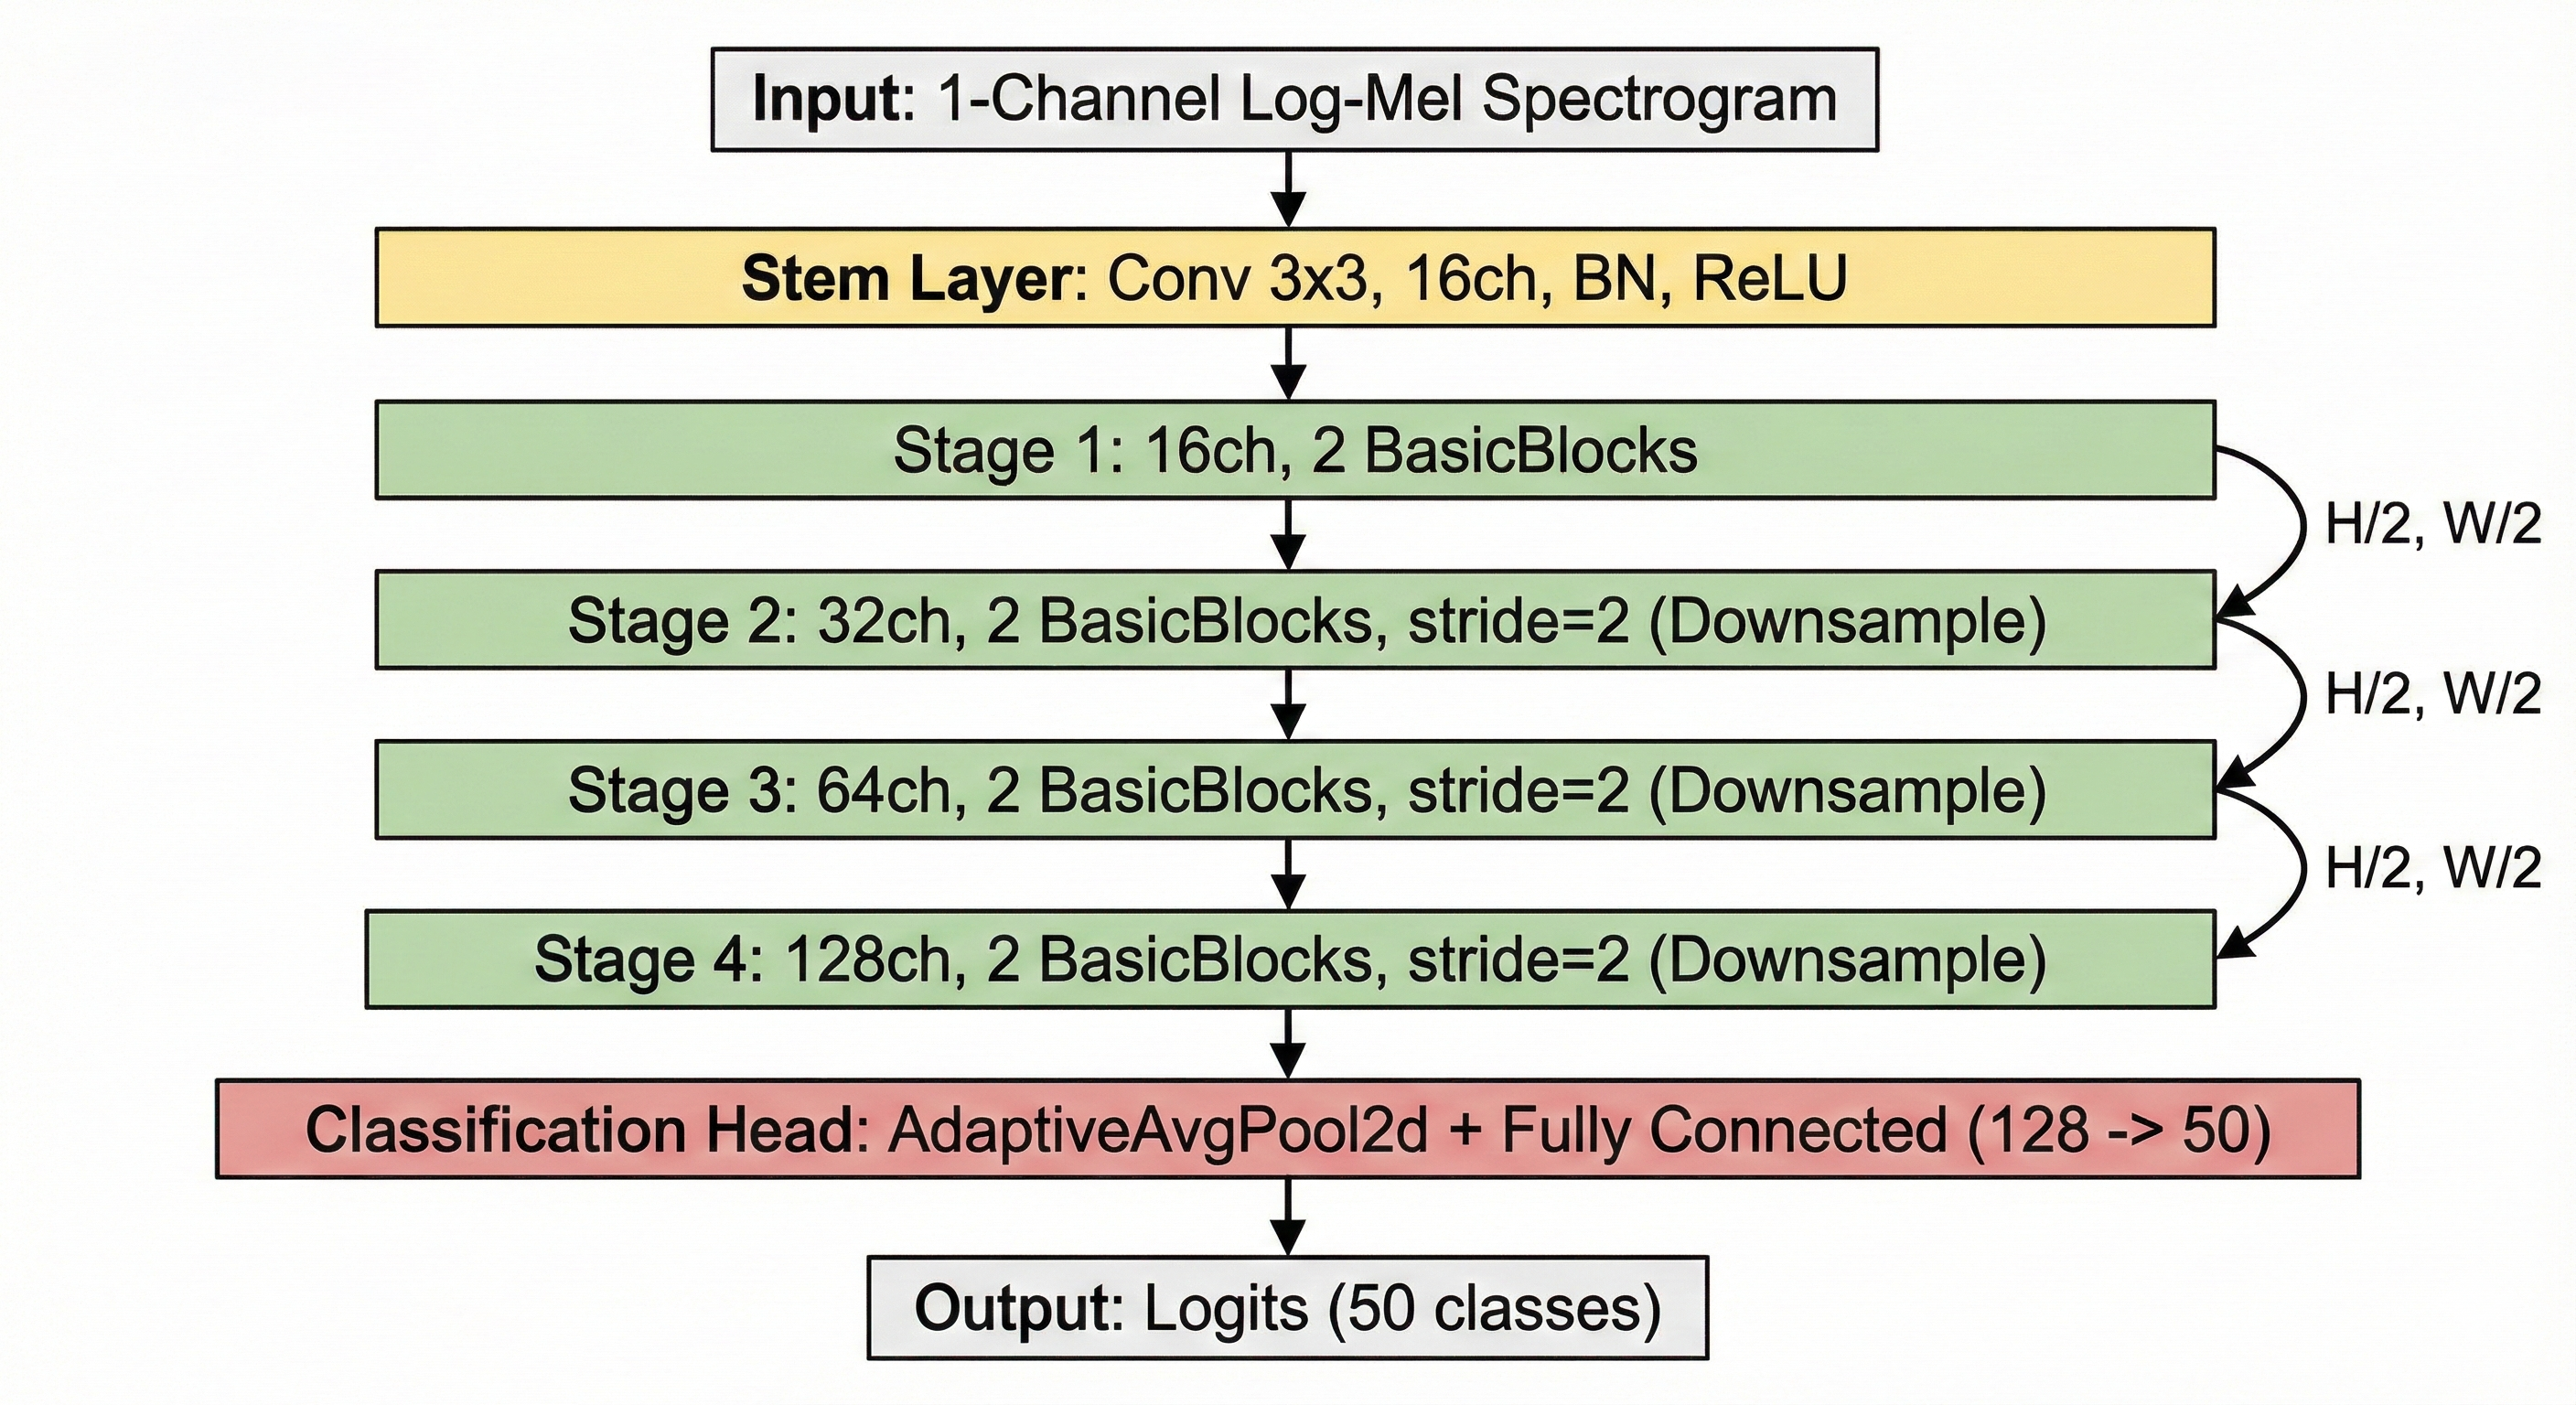
\includegraphics[width=0.75\textwidth]{figures/cnn.png}
    \caption{ResNet-Audio 模型架构}
    \label{fig:cnn_arch}
\end{figure}
\subsection{训练策略}
\begin{itemize}
    \item \textbf{特征输入}:40维Log-Mel频谱图。
    \item \textbf{优化器}:Adam,学习率 0.001。
    \item \textbf{损失函数}:交叉熵损失(CrossEntropyLoss)。
    \item \textbf{训练轮次}:50 Epochs。
    \item \textbf{批大小}:32。
\end{itemize}

\subsection{实验结果与分析}

我们同样进行了帧长与帧移的网格搜索,结果如表\ref{tab:classification_acc}所示。

\begin{table}[htbp]
\centering
\caption{CNN分类测试准确率 (Frame Length vs Hop Length)}
\label{tab:classification_acc}
\begin{tabular}{c|cccc}
\toprule
\multirow{2}{*}{Frame Length} & \multicolumn{4}{c}{Hop Length} \\
 & 256 & 512 & 1024 & 2048 \\
\midrule
512  & 0.6725 & 0.6975 & 0.7025 & 0.6450 \\
1024 & 0.7025 & 0.6950 & 0.7225 & 0.6700 \\
2048 & 0.6925 & 0.7150 & \textbf{0.7500} & 0.7200 \\
4096 & 0.6650 & 0.7000 & 0.7100 & 0.7000 \\
\bottomrule
\end{tabular}
\end{table}

\begin{figure}[htbp]
    \centering
    \includegraphics[width=0.7\textwidth]{../../outputs/results/run_20251221_003516/plots/cnn_history.png}
    \caption{CNN训练过程曲线(训练集Acc > 90\%,验证集Acc停滞在75\%,显示过拟合)}
    \label{fig:cnn_loss}
\end{figure}
% \begin{figure}[htbp]
%     \centering
%     \begin{subfigure}{0.48\textwidth}
%         \includegraphics[width=\linewidth]{../../outputs/results/run_20251221_003516/plots/cnn_history.png}
%         \caption{训练过程曲线}
%         \label{fig:cnn_loss}
%     \end{subfigure}
%     \begin{subfigure}{0.48\textwidth}
%         \includegraphics[width=\linewidth]{../../outputs/results/run_20251221_003516/plots/classification_grid_heatmap.png}
%         \caption{超参数热力图}
%         \label{fig:cnn_heatmap}
%     \end{subfigure}
%     \caption{CNN训练与超参数分析}
% \end{figure}

\textbf{结果分析:}
\begin{enumerate}
    \item \textbf{最优性能}:在帧长2048、帧移1024时达到最高准确率\textbf{75.00\%}。
    \item \textbf{2:1}:表现较好的组合(1024/512, 2048/1024)的帧长与帧移比值通常为2:1,这保证了50\%的帧重叠率,既保留了信息又避免了过度冗余。
    \item \textbf{过拟合现象}:从训练曲线(图\ref{fig:cnn_loss})可见,训练集准确率最终超过90\%,而测试集停滞在75\%,表明模型在小数据集上存在过拟合倾向。
\end{enumerate}

\section{大模型时代的音频理解}

为了探索音频理解的上限,我们引入了基于大规模预训练数据的模型。

\subsection{模型介绍}
\begin{itemize}
    \item \textbf{PANNs (Cnn14)}:在大规模音频数据集AudioSet(200万条)上预训练的CNN模型\cite{kong2020panns}。
    \item \textbf{AST (Audio Spectrogram Transformer)}:基于Vision Transformer架构,同样在AudioSet上预训练\cite{gong2021ast}。
    \item \textbf{CLAP (Contrastive Language-Audio Pretraining)}:在LAION-Audio-630K图文对上进行对比学习预训练,支持零样本分类\cite{wu2024clap}。
    \item \textbf{Gemini 3 Flash}:Google目前(2025年12月)的次旗舰多模态大语言模型,具备通用的多模态理解能力\cite{gemini3flash}。
\end{itemize}

\subsection{对比实验结果}
我们对比了自研模型与各基线模型的性能(见表\ref{tab:models_comparison})。迁移学习采用Linear Probe方式(冻结backbone,训练线性头)。

\begin{table}[htbp]
\centering
\caption{不同模型性能对比总表}
\label{tab:models_comparison}
\begin{tabular}{lllc}
\toprule
模型 & 方法 & 预训练数据 & 准确率 \\
\midrule
\textbf{ResNet (Ours)} & Supervised (Scratch) & None (仅ESC-50) & 75.00\% \\
Gemini Flash & Zero-shot LLM & Multimodal (Web) & 78.00\% \\
\textbf{Human Accuracy} & \textbf{Crowdsourcing} & \textbf{Biological Evolution} & \textbf{81.30\%} \cite{piczak2015esc} \\
PANNs & Transfer Learning & AudioSet (2M) & 90.50\% \\
CLAP (Zero-shot) & Zero-shot & LAION-Audio (630K) & 91.50\% \\
AST & Transfer Learning & AudioSet (2M) & 95.00\% \\
\textbf{CLAP (Transfer)} & \textbf{Transfer Learning} & \textbf{LAION-Audio (630K)} & \textbf{97.25\%} \\
\bottomrule
\end{tabular}
\end{table}

\textbf{深度洞察:}
\begin{itemize}
    \item \textbf{超人类的表现}:现代音频基础模型(CLAP, AST, PANNs)的准确率(>90\%)已经大幅超越了人类听觉的平均水平(81.30\%)。这表明在特定领域的分类任务上,“机器听觉”已经实现了对“生物听觉”的超越。
    \item \textbf{人类水平的门槛}:有趣的是,我们的自研小模型(75\%)和通用大模型Gemini 3 Flash(78\%)恰好处于接近人类水平但略低的区间。这说明达到人类的“直觉”水平相对容易,但要达到“专家”水平(>90\%)则需要大规模的领域专业训练数据。
    \item \textbf{多模态的威力}:CLAP利用文本语义引导音频特征学习,其Zero-shot能力(91.50\%)甚至超过了PANNs的监督迁移结果,这意味着模型真正理解了声音的语义。
\end{itemize}

\section{总结与思考}

本项目通过完整的系统实现与对比实验,不仅验证了算法的有效性,更揭示了音频处理技术发展的内在逻辑。

\subsection{不变的数学基石}
纵观从基础的MFCC到最前沿的AST、CLAP大模型,我们发现一个有趣的现象:尽管模型架构日新月异,但它们的输入端无一例外地都指向了\textbf{频谱图}。这深刻说明,\textbf{频域分析依然是连接物理声学与与机器智能的“通用语言”}。傅里叶变换(FFT)这一诞生于19世纪的数学工具,跨越了算法的代际更迭,依然是支撑现代人工智能大厦的底层基石。

\subsection{演进的特征范式}
通过对比不同模型的表现,我们清晰地看到了\textbf{表示学习(Representation Learning)}的三次范式跃迁:
\begin{itemize}
    \item \textbf{规则驱动 (DSP)}:如MFCC,依赖人工设计的物理和听觉规则,可解释性强(捕捉共振峰),但难以描述复杂的语义。
    \item \textbf{数据驱动 (Deep Learning)}:如ResNet,通过CNN自动提取频域纹理特征,性能大幅提升,但本质上仍是模式识别。
    \item \textbf{语义驱动 (Foundation Models)}:如CLAP,将声音映射到文本语义空间,实现了真正的“听音识意”,使得机器听觉超越了单纯的分类,具备了理解能力。
\end{itemize}

未来的音频技术,必将是“经典信号处理”与“大规模预训练”的深度共生。底层的物理模型提供精确的时频描述,上层的数据模型赋予其广义的语义理解,共同推动机器听觉向着“超人类”的智能水平迈进。

% \appendix
% \section{附录:代码与文件索引}
% \begin{itemize}
%     \item 项目根目录:\texttt{Audiofool934/dsp-final}
%     \item 核心DSP代码:\texttt{src/dsp/fft.py, stft.py, mfcc.py}
%     \item 检索任务结果:\texttt{outputs/results/run\_20251221\_003516/retrieval/}
%     \item 模型权重文件:\texttt{outputs/results/run\_20251221\_003516/models/}
%     \item 详细错误分析:\texttt{outputs/results/run\_20251221\_003516/errors/}
% \end{itemize}


\bibliographystyle{plain}
\bibliography{ref}

\end{document}
